\documentclass{report}
\usepackage[english]{babel}
\usepackage{array}
\usepackage{float}
\usepackage[dvipsnames]{xcolor}

\usepackage[most,many,breakable]{tcolorbox}
\usepackage{xcolor}

\definecolor{defBoxBorder}{HTML}{395144}
\newtcolorbox{defBox}{colback=white,colframe=defBoxBorder,arc=3pt, boxrule=0.5pt, drop fuzzy shadow, title=Definition}
\definecolor{thBoxBorder}{HTML}{AC8441}
\newtcolorbox{thBox}{colback=white,colframe=thBoxBorder,arc=3pt, boxrule=0.5pt, drop fuzzy shadow, title=Theorem}
\definecolor{noteBoxBorder}{HTML}{4E6C50}
\newtcolorbox{noteBox}{colback=white,colframe=noteBoxBorder,arc=3pt, boxrule=0.5pt, drop fuzzy shadow, title=Note}
\definecolor{axBoxBorder}{HTML}{AA5656}
\newtcolorbox{axBox}{colback=white,colframe=axBoxBorder,arc=3pt, boxrule=0.5pt, drop fuzzy shadow, title=Axiom/Postulate}
\definecolor{corBoxBorder}{HTML}{8B7E74}
\newtcolorbox{corBox}{colback=white,colframe=corBoxBorder,arc=3pt, boxrule=0.5pt, drop fuzzy shadow, title=Corollary}
\definecolor{lemBoxBorder}{HTML}{B99B6B}
\newtcolorbox{lemBox}{colback=white,colframe=lemBoxBorder,arc=3pt, boxrule=0.5pt, drop fuzzy shadow, title=Lemma}


\usepackage[spanish]{babel}
\usepackage[utf8x]{inputenc}
\usepackage{amsmath}
\usepackage{graphicx}
\usepackage[colorinlistoftodos]{todonotes}
\usepackage{enumitem}
\usepackage{listings}
\usepackage{verbatim}
\usepackage{eurosym}
\usepackage[export]{adjustbox}
\usepackage{amssymb}
\usepackage{bussproofs}
\usepackage{amsmath}
\usepackage{tikz}
\usepackage{xcolor}
\usepackage{listings}
\usepackage{titletoc}
\usepackage{hyperref}

\hypersetup{
  colorlinks=true,
  linkcolor=black,
  urlcolor=blue,
  citecolor=black
}

\newcommand{\coverPage}[6]{%
%----------------------------------------------------------------------------------------
%	COVER START
%----------------------------------------------------------------------------------------
\begin{titlepage}

    \newcommand{\HRule}{\rule{\linewidth}{0.5mm}}
    \newcommand{\department}{#1}
    \newcommand{\course}{#2}
    \newcommand{\titleValue}{#3}
    \newcommand{\subtitleValue}{#4}
    \newcommand{\authorName}{#5}

    \center

    %----------------------------------------------------------------------------------------
    %	HEADER
    %----------------------------------------------------------------------------------------
    
\includegraphics{images/logo_usa.png}
    \vspace{0.5cm}
    \textsc{\Large \department}\\[0.5cm]
    \textsc{\Large \course}\\[0.5cm]
    \vfill

    %----------------------------------------------------------------------------------------
    %	TITLE
    %----------------------------------------------------------------------------------------

    \HRule\\
    \Huge
    \textbf{\titleValue}\\[0.5cm]
    \Large
    \textbf{\subtitleValue}\\
    \HRule\\[0.5cm]

    %----------------------------------------------------------------------------------------
    %	AUTHOR AND DATE
    %----------------------------------------------------------------------------------------

    \vfill
    \Large
    \textit{\authorName}\\
    {\large \today}\\[2cm]

\end{titlepage}
%----------------------------------------------------------------------------------------
%	COVER END
%----------------------------------------------------------------------------------------
}

\begin{document}
    \coverPage{ Mathematics }{ Integral Calculus and Series }{ Integration }{ Techniques for finding antiderivatives. }{ Alexander Mendoza }{\today}
    \tableofcontents

    \pagebreak
    \chapter{ Integration }

    \section{Elemental antiderivatives}

    After providing the motivation for the integral, giving a proper definition of it and stating some of its applications, it's now worth studying effective ways to find antiderivatives and thus solving definite or indefinite integrals. We'll begin by providing a table with some antiderivatives for familiar functions. Let $n \in \mathbb{R}$.

    \begin{table}[H]
        \setlength{\extrarowheight}{10pt}
        \centering
        \begin{tabular}{|c|c|}
        \hline
        $f(x)$          & $\int f(x) \, dx$           \\ \hline
        $n$             & $nx+C$                      \\ \hline
        $x^n$           & $\frac{1}{n+1}x^{n+1} + C \text{ if } x \not = 1$ \\ \hline
        $\sin x$        & $-\cos x + C$               \\ \hline
        $\cos x$        & $\sin x + C$                \\ \hline
        $\sec^2x$       & $\tan x + C$                \\ \hline
        $\csc^2x$       & $-\cot x +C$                \\ \hline
        $\sec x \tan x$ & $\sec x +C$                 \\ \hline
        $\csc x \cot x$ & $-\csc x +C$                \\ \hline
        \end{tabular}%
        % }
    \end{table}

    Additionally, we know that

    $$\int mf(x) \,dx = m\int f(x) \,dx$$
    $$\int f(x) + g(x) \,dx = \int f(x) \,dx + \int g(x) \,dx$$

    \begin{Example}
        For the definite integral of a constant we have
        $$\int_{a}^{b}c\,dx = cb - ca$$
    \end{Example}

    \begin{Example}
        For the definite integral of a variable $x$ we have
        $$\int_{a}^{b}x\,dx = \int_{a}^{b}x^1\,dx = \left( \dfrac{1}{2}b^2 \right) - \left( \dfrac{1}{2}a^2 \right)$$
    \end{Example}

    \begin{Example}
        For the definite integral of $sin x$ we have

        $$\int_{a}^{b}\sin x \,dx = \left( -\cos b \right) - \left( -\cos a \right)$$
    \end{Example}

    \begin{Example}
        We can combine various rules together

        \begin{align*}
            \int_{a}^{b}(x^2 + x^3) \,dx &= \int_{a}^{b}x^2 \,dx + \int_{a}^{b}x^3 \,dx \\
            &= \left( \frac{b^3}{3} - \frac{a^3}{3} \right) + \left( \frac{b^4}{4} - \frac{a^4}{4} \right)
        \end{align*}
    \end{Example}

    Knowing these rules, we can now find an antiderivative for a considerable amount of functions which include all of the polynomials. However, for more complicated functions such as product of functions or composed functions we need some other tools, we will now state such tools.

    \begin{thBox}
        \textit{\textbf{Integration by Parts}}. if $f'$ and $g'$ are continuous, then

        $$\int fg' = fg - \int f'g \text{ or}$$
        $$\int f(x)g'(x) dx = f(x)g(x) - \int f'(x)g(x)dx \text{ and}$$
        $$\int_{a}^{b} f(x)g'(x) dx = f(x)g(x)\Big|_a^b - \int_a^b f'(x)g(x)dx$$
    \end{thBox}

    \begin{center}
        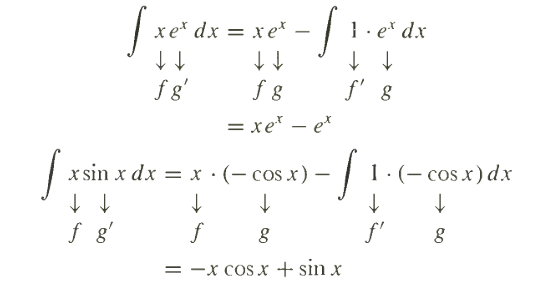
\includegraphics[width=1\textwidth]{images/productrule.png}
    \end{center}

    
\end{document}
